\section{Test mit zusätzlichen Addiererklauseln}

sinnvoll, da diese einen großteil ausmachen und den Sat-Solver ausbremsen könnten?

\TODO{erledigen}

\begin{figure}[!h]
  \centering
  \begin{minipage}[c]{0.45\textwidth}
  \begin{flushleft}Gesamtdauer ohne XOR: 410:59:52\end{flushleft}
  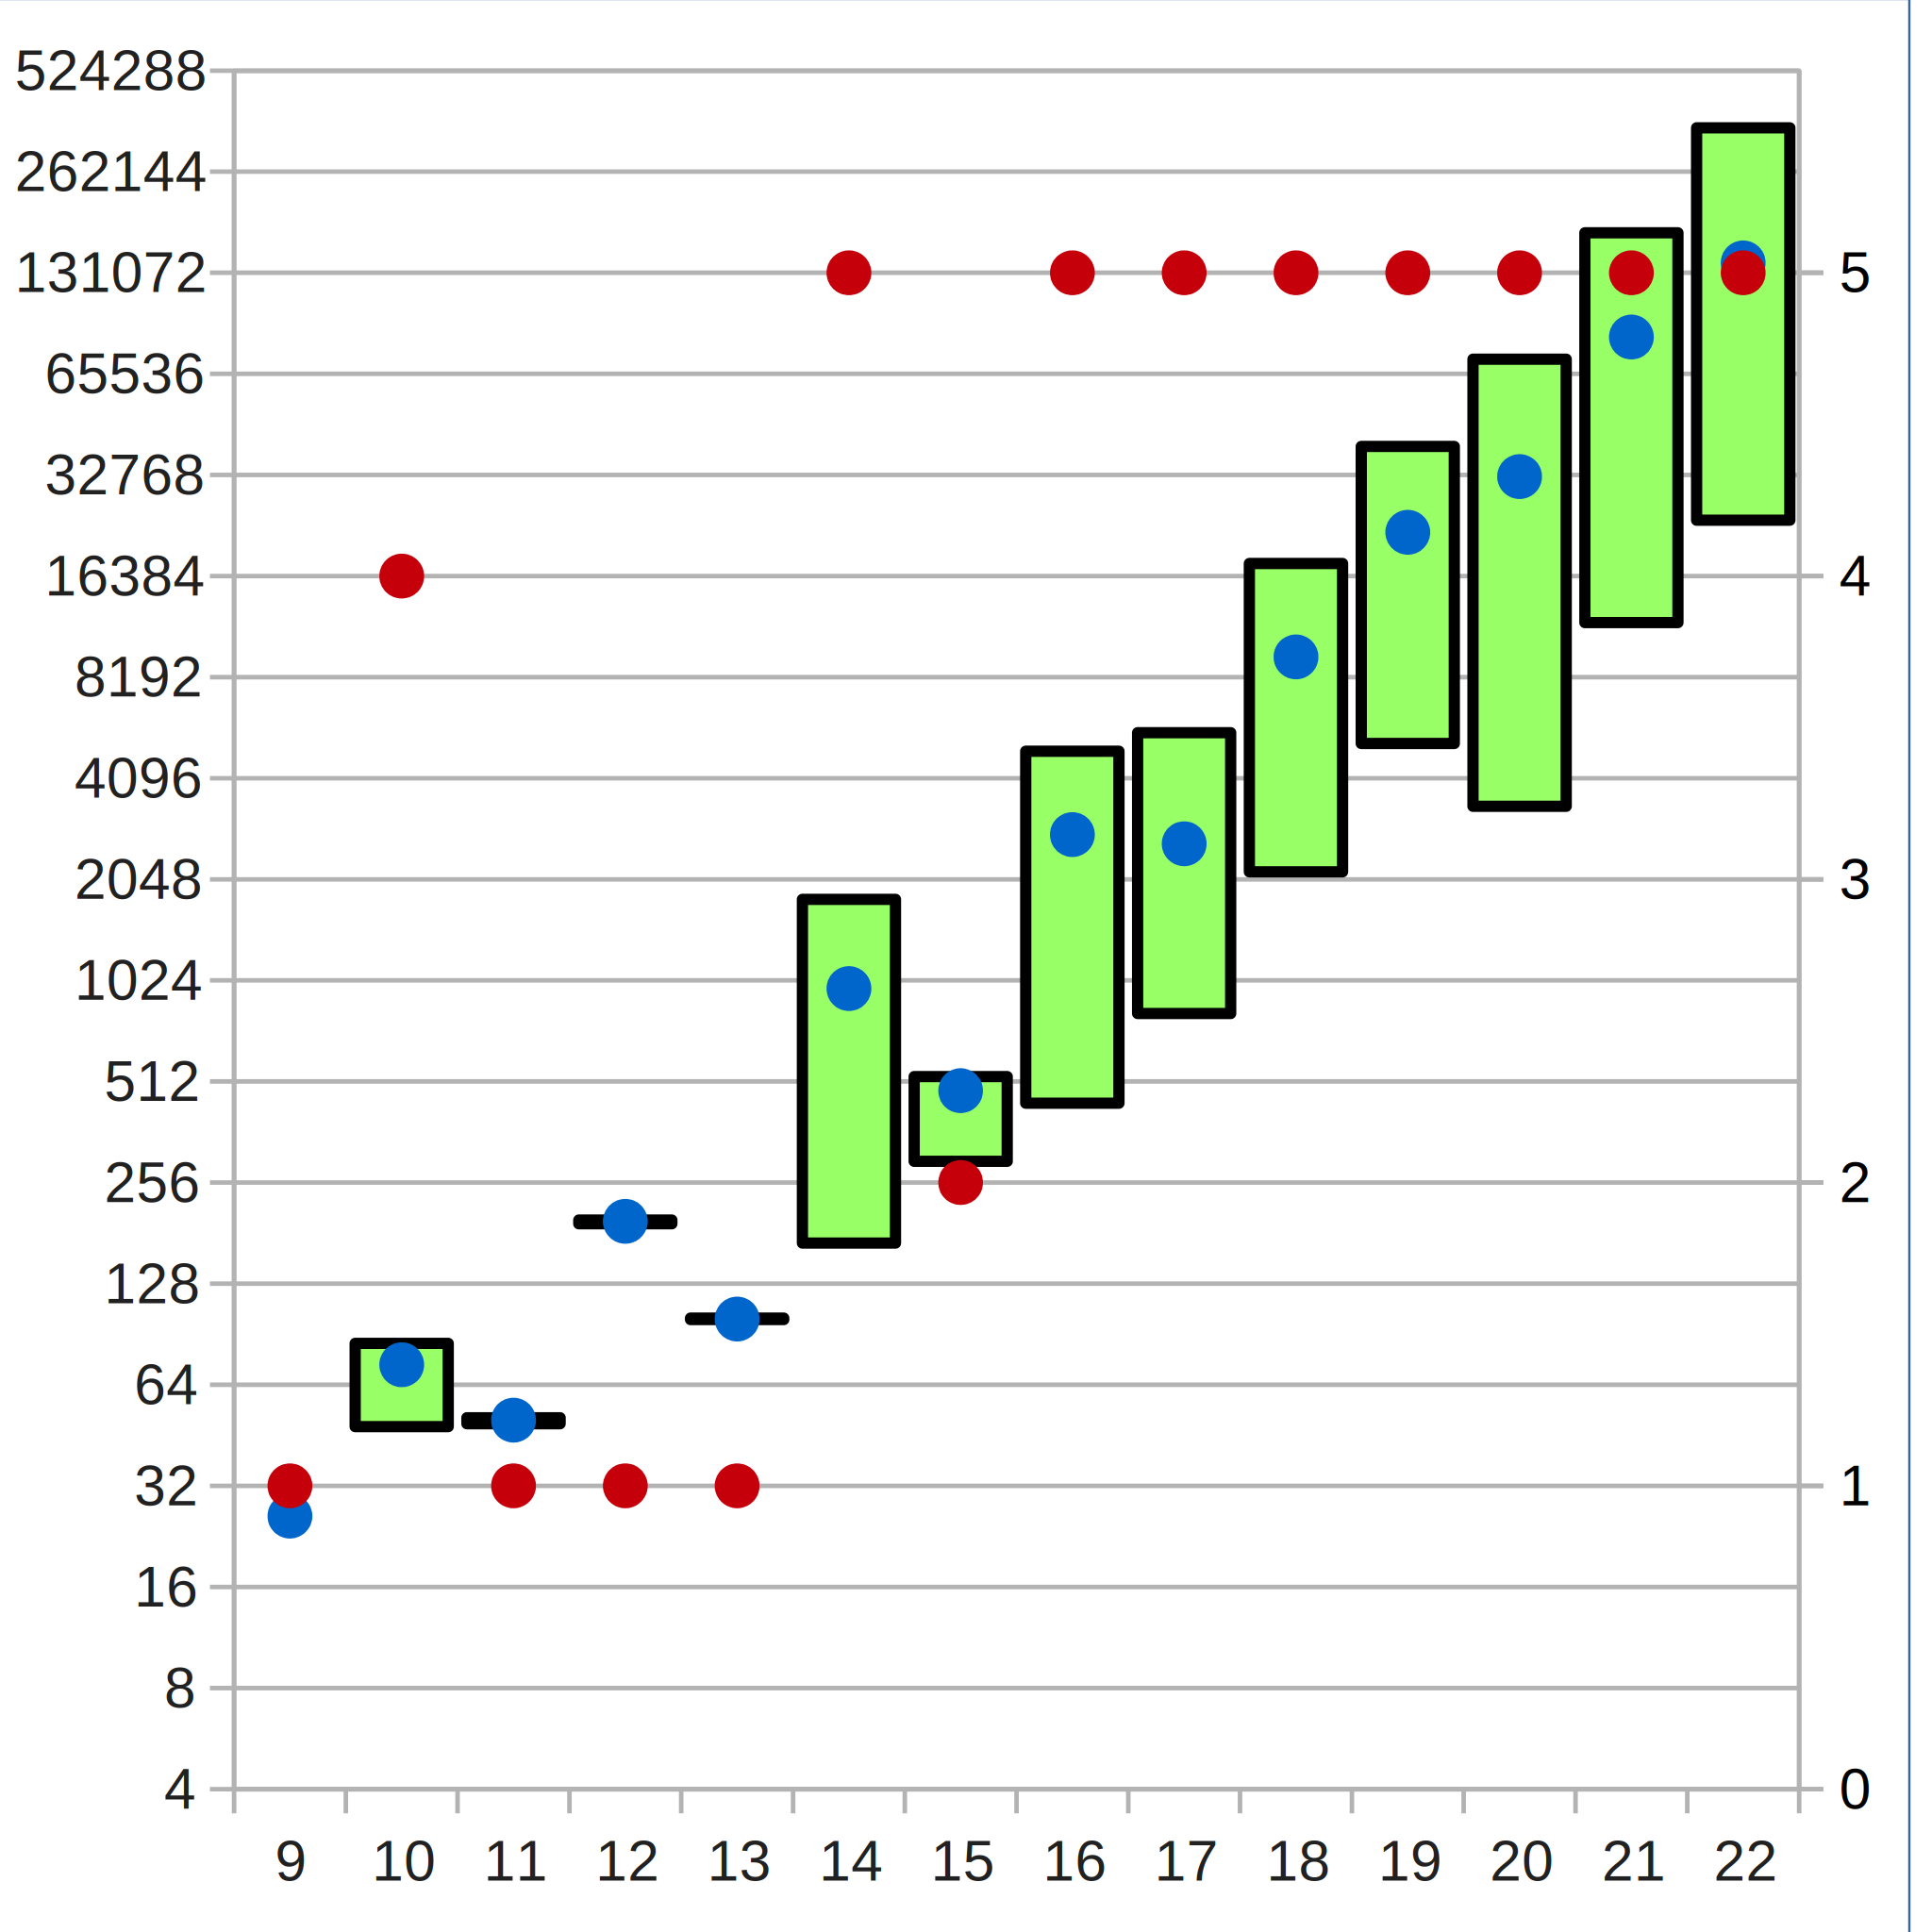
\includegraphics[scale=0.55]{images/data_add_knf}
  \end{minipage}
  \begin{minipage}[c]{0.09\textwidth}
  ~~
  \end{minipage}
  \begin{minipage}[c]{0.45\textwidth}
  \begin{flushleft}Gesamtdauer mit XOR: 491:53:48\end{flushleft}
  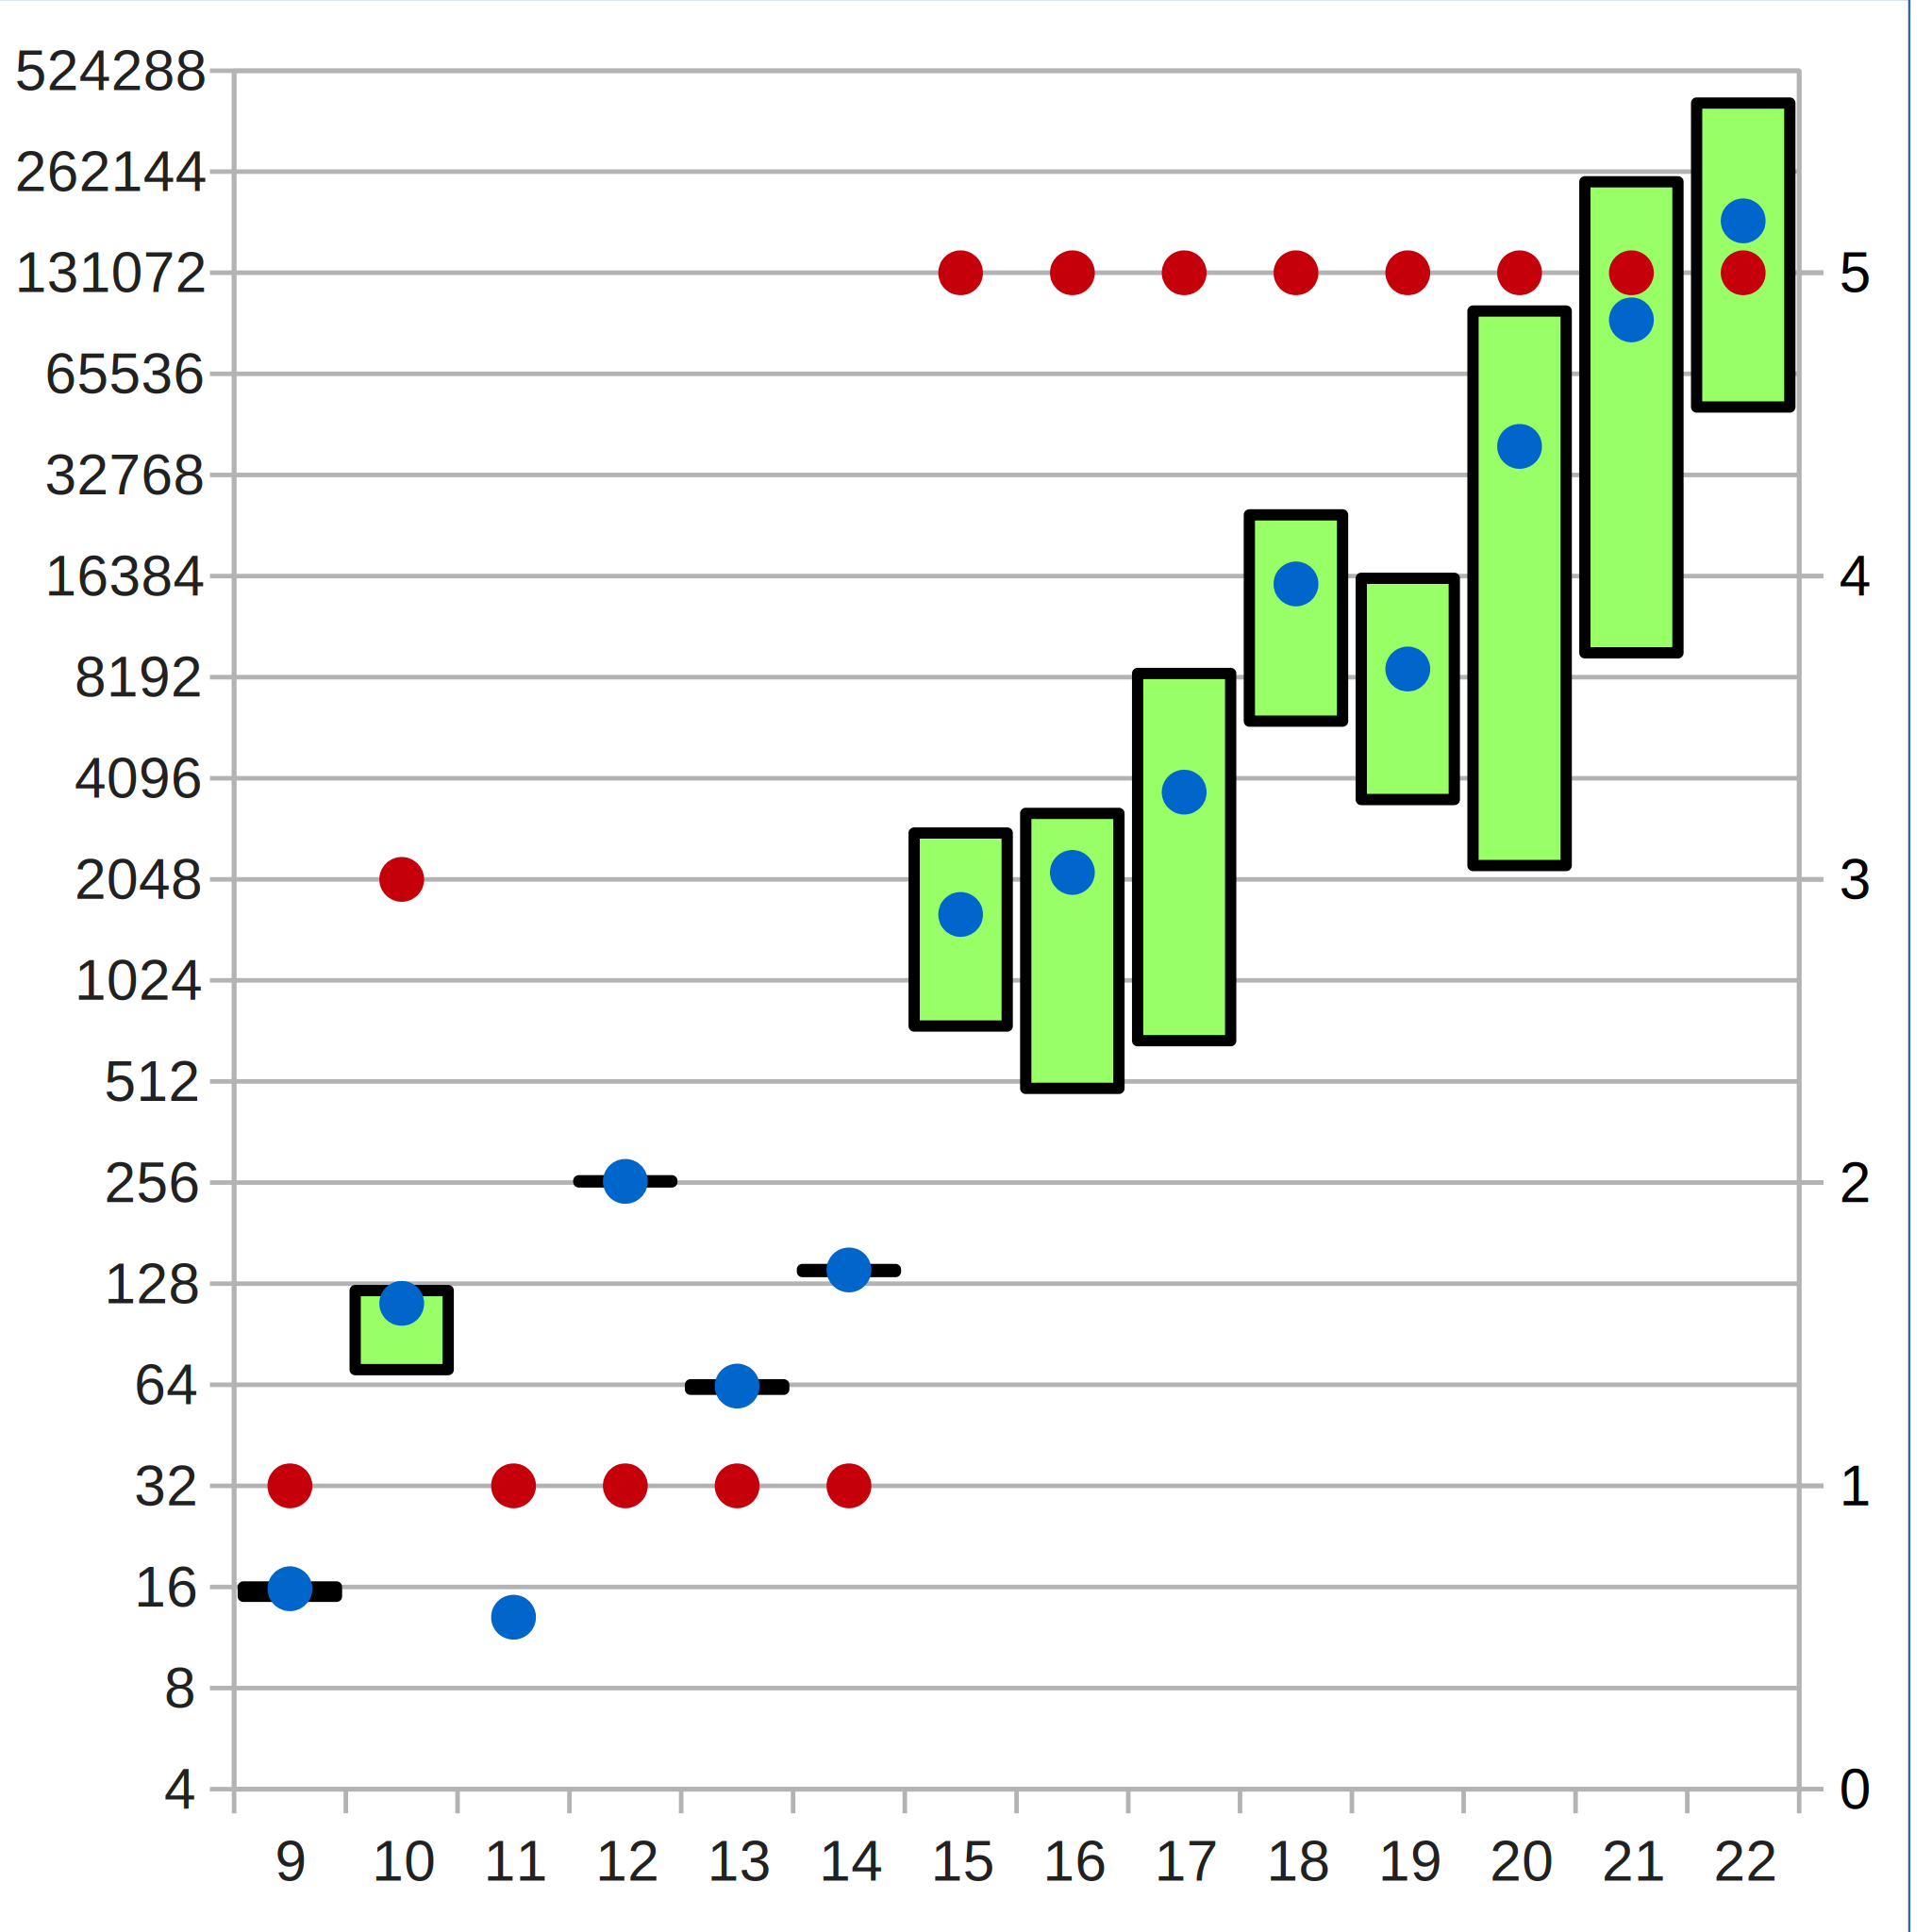
\includegraphics[scale=0.55]{images/data_add_xor}
  \end{minipage}
  \caption{TODO}
  \label{fig:data_add}
\end{figure}